\section{방법}
\label{sec:method}

% 한국어 구조 초안. 수식과 구성 요소의 경계는 Outline.md를 따르며,
% 구현 세부 문장과 인용은 영문 본문 단계에서 보강한다.

\subsection{문제 설정과 목표}
\label{sec:problem_setup}

$\mathcal{S}=\{x_j^n\}_{j=1}^{N}$를 few-shot normal support set, $x^q$를 query
image라 하자. 목표는 normal support만으로 fitting과 통계 추정을 수행하여 dense
continuous anomaly map $A(x^q)$을 생성하는 것이다. Query label은 feature extractor, Flow,
메모리, 통계량 및 하이퍼파라미터를 갱신하는 데 사용하지 않는다.

관측 점수는 다음의 개념적 관계로 구성한다.
\begin{equation}
  s_{\mathrm{obs}}(x)\approx s_{\mathrm{anom}}(x)+b_{\mathrm{shift}}(x),
  \label{eq:shift_score}
\end{equation}
여기서 $b_{\mathrm{shift}}$는 정상적인 support--query shift가 anomaly evidence에 유입된
항을 의미한다. 이는 정확한 확률적 분해가 아니라 연구 가설이다. 목표는 실제
이상 반응을 억제하지 않으면서 분포 변화로 유발된 정상 반응을 줄이는 것이다.
support-calibrated threshold $\tau_{\mathcal S}$에 대해 다음 두 비율을 함께 평가한다.
\begin{equation}
  \Pr_{o\sim P_Q^N}[s_{\mathcal S}(o)>\tau_{\mathcal S}]
  \quad\text{및}\quad
  \Pr_{o\sim P_Q^A}[s_{\mathcal S}(o)>\tau_{\mathcal S}].
  \label{eq:normal_anomaly_rates}
\end{equation}

\subsection{외재적 강건성 스택}
\label{sec:method_overview}

제안 방법은 few-shot support--query distribution shift에서 발생하는
\cref{eq:evidence_degradation}의 세 가지 anomaly evidence 문제에 각각 대응하는
외재적 강건성 스택이다. Foundation backbone은 전체 과정에서 동결하며, normal
support만을 사용해 PPD bias field와 normalizing flow를 fitting하고 static latent
bank를 구성한다. 이후 모든 support-fitted component를 고정한 상태에서 shifted
query의 representation, reference comparison 및 spatial evidence를 순차적으로
보정한다.

전체 처리 흐름은 다음과 같다.
\begin{equation}
  \begin{aligned}
    H
      &\xrightarrow{\text{PPD}} \widehat H
       \xrightarrow{\text{Flow-LatentBank}} d_z \\
      &\xrightarrow{\text{weak NLL}} A_{\mathrm{coarse}}
       \xrightarrow{\text{RGB Guide}} A_{\mathrm{rgb}}.
  \end{aligned}
  \label{eq:pipeline}
\end{equation}
각 구성요소와 증거 문제의 대응은
\begin{equation}
  \begin{aligned}
    b_{\mathrm{rep}} &\longrightarrow \mathrm{PPD},\\
    b_{\mathrm{ref}} &\longrightarrow \mathrm{Flow\text{-}LatentBank},\\
    d_{\mathrm{sp}}  &\longrightarrow \mathrm{RGB\ Guide}.
  \end{aligned}
  \label{eq:problem_component_mapping}
\end{equation}
로 요약된다. PPD는 normal support에서 반복되는 position-dependent descriptor
bias를 추정하고 support와 query에 대칭적으로 적용하여 representation mismatch를
완화한다. Static Flow-LatentBank는 보정된 normal support를 standardized latent
space로 변환하고, query patch를 변환된 실제 support instance와 비교하여 reference
geometry를 안정화한다. RGB Guide는 coarse anomaly evidence를 현재 query RGB에
보존된 boundary와 local contrast에 맞게 정제한다.

방법은 support fitting과 query inference의 두 단계로 동작한다. Support fitting
단계에서는 PPD bias field, normalizing flow, static latent bank 및 support statistics를
normal support만으로 구성한다. Query inference에서는 저장된 변환과 통계량만을
사용하며, foundation representation을 갱신하거나 query label을 사용하거나 memory를
갱신하지 않는다. 즉, test-time adaptation을 수행하는 대신 normal support로 미리
구성하고 고정한 보정 경로를 통해 shifted query의 anomaly evidence를 안정화한다.

\subsection{Patch Positional Debiasing}
\label{sec:ppd}

DVT는 ViT feature에 image content와 독립적으로 반복되는 position-related
artifact가 존재할 수 있음을 보이고, transformed view와 neural field를 이용해
semantic feature와 artifact field를 분해한다~\cite{yang2024dvt}. 이 관찰에
착안하여, PPD는 few-shot normal support에 적용할 수 있는 경량
support-statistical calibration을 구성한다. 원래 DVT의 cross-view decomposition과
달리, PPD는 normal support로부터 위치마다 반복되는 descriptor component를 직접
추정한다.

$H_j^s(u)$를 $j$번째 normal support의 patch-grid position $u$에서 얻은
descriptor라 하자. 먼저 각 위치의 support 평균을 계산하고, support와 query에서
이를 대칭적으로 제거한다.
\begin{align}
  \mu_{\mathrm{pos}}(u)
    &= \frac{1}{N}\sum_j H_j^s(u), \\
  \widetilde H(u)
    &= H(u)-\mu_{\mathrm{pos}}(u).
  \label{eq:ppd_centering}
\end{align}
$\mu_{\mathrm{pos}}(u)$는 위치 $u$에서 support 전반에 반복되는 descriptor
component를 나타낸다. 이를 제거한 support residual의 채널별 표준편차를
\begin{equation}
  \sigma_{\mathcal S}
    =\operatorname{Std}_{j,u}\!\left[\widetilde H_j^s(u)\right]
  \label{eq:ppd_scale}
\end{equation}
로 추정하고, Flow에 전달되는 최종 feature를
\begin{equation}
  \widehat H(u)
    =\frac{\widetilde H(u)}{\max(\sigma_{\mathcal S},\epsilon)}
  \label{eq:ppd_standardization}
\end{equation}
로 정의한다. 모든 연산은 feature channel별로 적용하며, $\epsilon$은 수치적
안정성을 위한 작은 상수이다. Position-wise centering은 PPD의 고유 보정이고,
channel-wise standardization은 PPD on/off를 포함한 모든 Flow 기반 variant에
공통으로 적용되는 입력 전처리이다. 여기서는 Flow에 전달되는 calibrated feature를
한 번에 명확히 하기 위해 두 단계를 함께 기술한다.

Layout, scale 또는 viewpoint shift로 동일한 normal content가 support와 query에서
서로 다른 patch position에 놓이면, position-conditioned component의 차이가
descriptor mismatch에 유입될 수 있다. PPD는 이 반복 component를 양쪽
representation에서 동일하게 억제하여 position-dependent mismatch를 완화한다.
다만 정렬된 support에서는 $\mu_{\mathrm{pos}}(u)$가 positional artifact뿐 아니라
반복적인 normal object structure도 포함할 수 있다. 따라서 PPD는 두 성분의 완전한
분리를 보장하지 않으며, support에서 추정한 position-conditioned component를
억제하는 보정으로 주장 범위를 제한한다.

\subsection{Static Flow-LatentBank: Likelihood-trained Latent Encoder}
\label{sec:latent_bank}

Finite support로 구성한 reference는 normal feature distribution의 일부만을
표본화하기 때문에, finite reference는 raw feature space에서 normal distribution을
불균일하게 포괄할 수 있다. Support--query distribution shift가 발생하면 이러한
제한된 coverage와 shifted query 사이의 geometry mismatch가 더욱 두드러질 수 있으며,
그 결과 raw-space nearest-neighbor distance의 신뢰성이 저하될 수 있다. 이를
완화하기 위해 PPD로 보정한 normal support patch에 invertible patch-wise
affine-coupling MLP Flow $f_\theta$를 적합한다. Flow는 change-of-variables에 따른
support patch의 likelihood를 최대화하여, 이를 standard Gaussian base distribution으로
매핑하도록 학습된다.
\begin{equation}
  \ell_{\mathrm{NF}}(\widehat h)
    =\frac{1}{2}\lVert f_\theta(\widehat h)\rVert_2^2
     -\log\left|\det J_{f_\theta}(\widehat h)\right|+C,
  \label{eq:flow_nll}
\end{equation}
여기서 $J_{f_\theta}$는 $f_\theta$의 Jacobian이며, base distribution은 standard
Gaussian이다. 이 likelihood objective를 통해 $f_\theta$는 support distribution의
방향별 scale과 local density를 반영하는 invertible reparameterization을 학습한다.

본 방법에서 Flow의 주된 역할은 likelihood 자체로 anomaly를 판정하는 것이 아니라,
normal comparison을 위해 support와 query를 support-conditioned coordinate system으로
매핑하는 데 있다.
Likelihood를 직접 anomaly score로 사용하는 일반적인 flow-based anomaly
detection~\cite{gudovskiy2022cflow}과 달리, 학습된 $f_\theta$를
\emph{latent encoder}로 사용한다. 학습이 완료되면 normal support patch를 Flow로
변환하고, 해당 latent representation을 static latent bank에 저장한다.
\begin{equation}
  z=f_\theta(\widehat h),
  \qquad
  \mathcal{M}_z=\{f_\theta(\widehat h_{j,u}^s)\}_{j,u}.
  \label{eq:latent_bank}
\end{equation}
Query patch $i$도 동일한 encoder로 변환하며, primary anomaly score는 static
support bank까지의 latent 1-NN distance로 정의한다.
\begin{equation}
  d_z(i)=\min_{m\in\mathcal{M}_z}\|z_i^q-m\|_2.
  \label{eq:latent_nn}
\end{equation}
즉, test-time의 query patch 역시 동일한 $f_\theta$로 변환한 뒤, 학습된 likelihood
자체가 아니라 latent bank 내 실제 normal support와의 거리를 주된 anomaly
evidence로 사용한다. Flow latent representation의 구체적인 효과와
distribution shift에서의 역할은 \cref{sec:experiments}의 비교 실험과 component
ablation을 통해 분석한다.

\subsection{RGB Guide: Query-native Spatial Restoration}
\label{sec:rgb_guide}

patch-level coarse map은 semantic anomaly evidence를 제공하지만, token 내부의
정확한 boundary와 local structure를 표현하기 어렵다. 특히 layout, scale 및
viewpoint shift로 anomaly와 주변 구조가 support와 다른 위치와 크기로 나타나면,
고정 patch grid에서 생성된 coarse response가 실제 query의 경계를 가로질러 확산될
수 있다. RGB Guide는 support의 spatial pattern을 다시 참조하는 대신, 현재 query에
남아 있는 image-level edge를 이용해 coarse anomaly evidence를 정제한다.

구체적으로 query RGB image를 grayscale guidance $I^q\in[0,1]$로 변환한다.
$P$는 \cref{eq:coarse_score}의 patch score를 2차원 patch grid에 배치하고 image
space로 upsample한 $A_{\mathrm{coarse}}$에 image별 min--max normalization을 적용한
입력 score map이다. 두 입력을 각각 반 해상도로 축소한 뒤, 각 local window
$\omega_k$에서 정제된 score가 guidance의 선형 변환으로 표현된다고 가정한다.
\begin{equation}
  Q_i=a_k I_i^q+b_k, \qquad i\in\omega_k.
  \label{eq:guided_local_model}
\end{equation}
계수 $a_k$와 $b_k$는 별도의 학습이나 iterative optimization 없이, 각 window에서
local linear output이 입력 coarse score $P$를 근사하도록 다음 ridge regression
목적함수를 최소화하여 결정한다.
\begin{equation}
  \min_{a_k,b_k}
  \frac{1}{|\omega_k|}\sum_{i\in\omega_k}
  \left(a_k I_i^q+b_k-P_i\right)^2+\epsilon a_k^2.
  \label{eq:guided_objective}
\end{equation}
첫 번째 항은 RGB guidance만으로 새로운 response를 생성하지 않도록, refined
response $a_k I_i^q+b_k$를 이미 계산된 anomaly evidence $P_i$에 결속하는 data
fidelity term이다. 두 번째 항은 RGB variance가 작거나 $I^q$와 $P$의 관계가
불안정한 window에서 slope $a_k$가 과도하게 커지는 것을 억제한다. 따라서 이
목적함수는 RGB edge를 anomaly evidence로 직접 추가하는 대신, 기존 coarse
evidence를 유지하면서 그 spatial transition만 query의 local image structure에
조건화한다. 평균 squared error를 사용했기 때문에 regularization strength
$\epsilon$은 window 크기에 의존하지 않으며, 위 목적함수의 해는 window 내부의
local statistics를 이용해 다음과 같이 닫힌 형태로 계산된다.
\begin{equation}
  a_k=\frac{\operatorname{Cov}_{\omega_k}(I^q,P)}
             {\operatorname{Var}_{\omega_k}(I^q)+\epsilon},
  \qquad
  b_k=\mu_{P,k}-a_k\mu_{I,k},
  \label{eq:guided_coefficients}
\end{equation}
여기서 $\mu_{I,k}$와 $\mu_{P,k}$는 각각 $\omega_k$에서의 guidance 및 coarse
score 평균이다. $a_k$는 RGB intensity와 coarse score의 local covariance를 RGB
variance와 regularization으로 나눈 값이므로, 단순한 RGB edge의 크기가 아니라 두
신호가 함께 변하는 정도를 나타낸다. $b_k$는 local linear output의 평균이 coarse
score의 평균 $\mu_{P,k}$와 일치하도록 정하는 intercept이다. 따라서 RGB가 변해도
$P$가 함께 변하지 않으면 $a_k$는 0에 가까워져 해당 edge가 anomaly boundary로
직접 전환되지 않는다. 반대로 두 신호가 함께 변하면 $a_k$가 그 관계를 반영하여
score transition을 query boundary에 맞춘다. 각 pixel은 여러
overlapping window에 포함되므로, 해당 pixel을 포함하는 window의 계수를 평균하여
최종 guided response를 계산한다.
\begin{equation}
  Q_i=\bar a_i I_i^q+\bar b_i,
  \quad
  \bar a_i=\frac{1}{|\Omega_i|}\sum_{k:i\in\omega_k}a_k,
  \quad
  \bar b_i=\frac{1}{|\Omega_i|}\sum_{k:i\in\omega_k}b_k,
  \label{eq:guided_aggregation}
\end{equation}
여기서 $\Omega_i$는 pixel $i$를 포함하는 local window의 집합이다. 즉, $P$는
Flow-LatentBank에서 이미 생성된 coarse anomaly evidence이며, $Q$는 $P$와 query
guidance $I^q$의 local statistics로부터 계산되는 refined response이다.
따라서 guidance가 평탄한 영역에서는 coarse response를 국소적으로 평활화하고,
RGB intensity가 급격히 변하면서 coarse score와 local covariance를 갖는 위치에서는
score transition을 보존한다. 이는 RGB edge를 새로운 anomaly evidence로 추가하는
것이 아니라, 기존 coarse evidence의 spatial propagation을 query의 관측 구조에
조건화하는 과정이다.

고정 guided filter $\mathcal{G}$는 반 해상도에서 radius $8$과
$\epsilon=0.01$을 사용한다. Filtering된 결과는 원래 coarse score 범위로
de-normalize하고 bilinear interpolation으로 native resolution에 복원한다. 전체
과정은 continuous map에 적용되며 thresholding과 binary morphology보다 먼저
수행된다. 정답이나 anomaly label을 사용하지 않고 backbone, Flow, latent bank 및
support statistics도 갱신하지 않는다. 다만 모든 RGB edge가 anomaly boundary와
일치하는 것은 아니므로, RGB Guide의 역할은 anomaly localization을 새로 생성하는
것이 아니라 이미 존재하는 coarse evidence의 boundary alignment를 보조하는 것으로
제한한다.

\begin{figure*}[t]
  \centering
  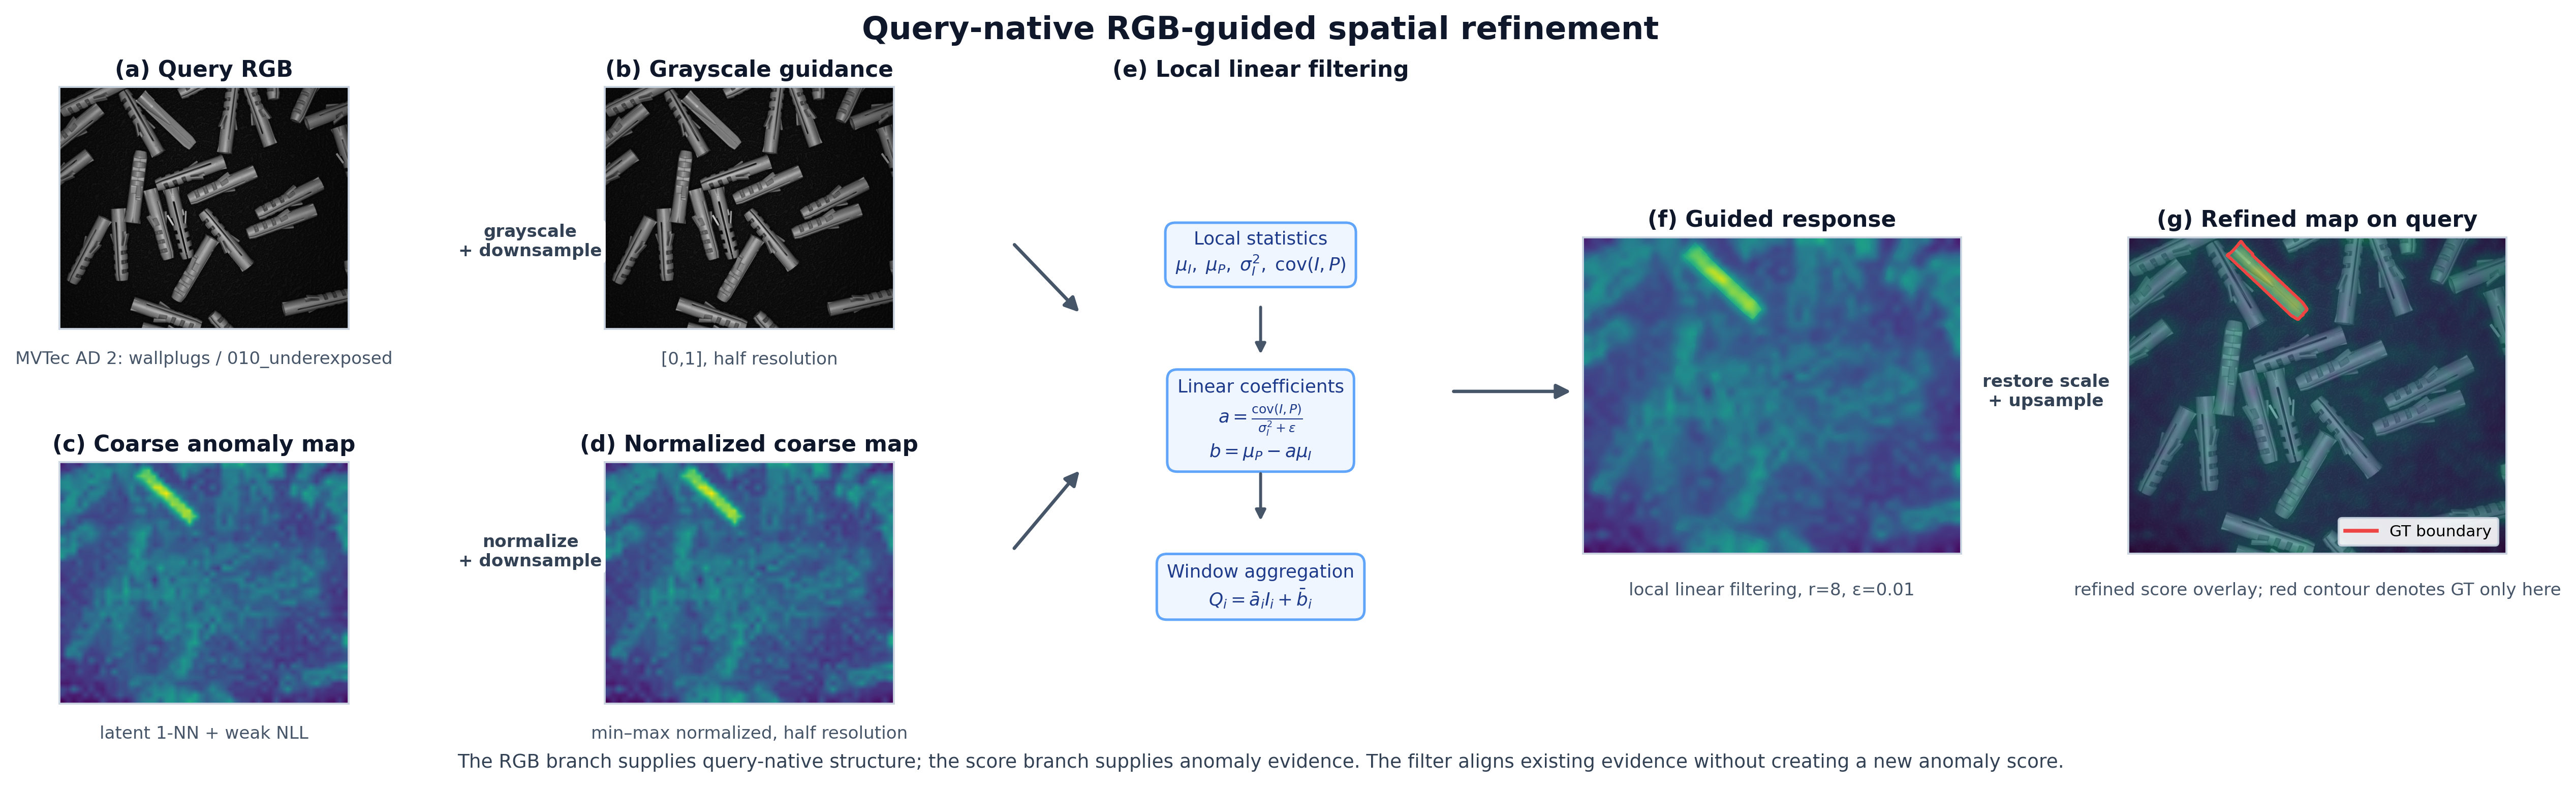
\includegraphics[width=\textwidth]{../figures/rgb_guide_process.pdf}
  \caption{MVTec AD 2의 \texttt{wallplugs/010\_underexposed} query sample을 이용한
  RGB Guide 처리 과정.
  Query RGB에서 얻은 grayscale guidance와 normalized coarse anomaly map을 각각 반
  해상도로 구성한다. Local window에서 guidance와 score의 mean, variance 및
  covariance를 계산하여 선형 계수 $a,b$를 구하고, overlapping window의 계수를
  평균하여 guided response를 생성한다. 이 response는 원래 score range로 복원한 뒤
  native resolution으로 upsample한다. 마지막
  panel의 score overlay와 빨간 GT contour는 spatial alignment를 시각화하기 위한
  것이다. GT는 이 마지막 panel에만 표시하며 guided filtering과 scoring에는 사용하지
  않는다.}
  \label{fig:rgb_guide_process}
\end{figure*}

\subsection{Final Anomaly Scoring Mechanism}
\label{sec:final_scoring}

최종 scoring mechanism은 latent 1-NN distance, weak density correction 및 RGB
Guide를 순서대로 결합한다. Primary anomaly evidence는
\cref{eq:latent_nn}의 latent distance $d_z(i)$이다. Flow likelihood는 직접적인
detector가 아니라, latent distance가 포착하지 못한 낮은 support likelihood를
보완하는 auxiliary signal로만 사용한다. 이를 위해 support patch에서 추정한 NLL
통계를 기준으로 query NLL의 양의 tail만 남긴다.
\begin{equation}
  r_{\mathrm{NF}}(i)=\operatorname{ReLU}\!\left(
    \frac{\ell_{\mathrm{NF}}(\widehat h_i^q)-\mu_{\mathrm{NF}}^s}
         {\max(\sigma_{\mathrm{NF}}^s,10^{-6})}
  \right).
  \label{eq:weak_nll}
\end{equation}
분모의 하한은 수치 안정성을 위한 것이며, weak density weight $\lambda_{\mathrm{NF}}=0.25$를
사용해 patch-level coarse score를 구성한다.
\begin{equation}
  s_{\mathrm{coarse}}(i)
    =d_z(i)+\lambda_{\mathrm{NF}}r_{\mathrm{NF}}(i).
  \label{eq:coarse_score}
\end{equation}
Coarse score를 patch grid에서 image resolution으로 upsample한 결과를
$A_{\mathrm{coarse}}$라 하면, 최종 continuous anomaly map은 현재 query RGB를
guide로 적용하여 얻는다.
\begin{equation}
  A_{\mathrm{rgb}}
    =\mathcal{G}(A_{\mathrm{coarse}},I_{\mathrm{RGB}}^q).
  \label{eq:rgb_guide}
\end{equation}
즉, likelihood는 latent encoder의 학습 objective이자 약한 보조 evidence로만
사용되고, latent 1-NN이 primary score를 구성하며, RGB Guide가 이를 pixel-level
spatial evidence로 복원한다. 이후 thresholding과 morphology는 이 continuous map에
적용한다.
